% Chapter 4

\chapter{Design and Implementation} % Main chapter title

\label{desi} % For referencing the chapter elsewhere, use \ref{desi}

\lhead{Chapter 4. \emph{Design and Implementation}} % This is for the header on each page - perhaps a shortened title
The inclusion of game schemes and elements in AnkiDroid required an analysis of its original design. The purpose was finding suitable parts in the structure of the application to integrate gamification components. Once these parts were found, the next step was to set an initial gamification strategy to modify the application. Later, it was necessary to design an approach to include a casual game. Such an approach needed to define a scheme to link the game to reviewing flashcards by means of the initial gamification strategy as seen in Figure \ref{fig:game-elem-cards}. Finally, it was necessary to consider user interface aspects for a smooth integration of the overall solution.

\begin{figure}[htb]
    \vskip 5mm
        \begin{center}
            
\includegraphics[scale=0.3]{./Figures/design.png}
            \caption{High level view of the design components and their relationships.}
            \label{fig:game-elem-cards}
        \end{center}
    \vskip -5mm
\end{figure}


%----------------------------------------------------------------------------------------
\section{Components of interest in AnkiDroid}
\label{desi-components-interest}
AnkiDroid is a mature application with a clear structure and well-defined logic. It has a user interface that follows the best design principles for mobile development. Despite its multiple features and functionalities, the core element is the flashcard reviewer. Here is where the application allows the users to benefit from the effects of spaced repetition. The available interactions to review flashcards permit the user to progress by checking the front of a flashcard (question), revealing its back (answer), and assessing it, which automatically leads to a new flashcard as seen in Figure \ref{fig:front-back-assess}.

\begin{figure}[htb]
    \vskip 5mm
        \begin{center}
            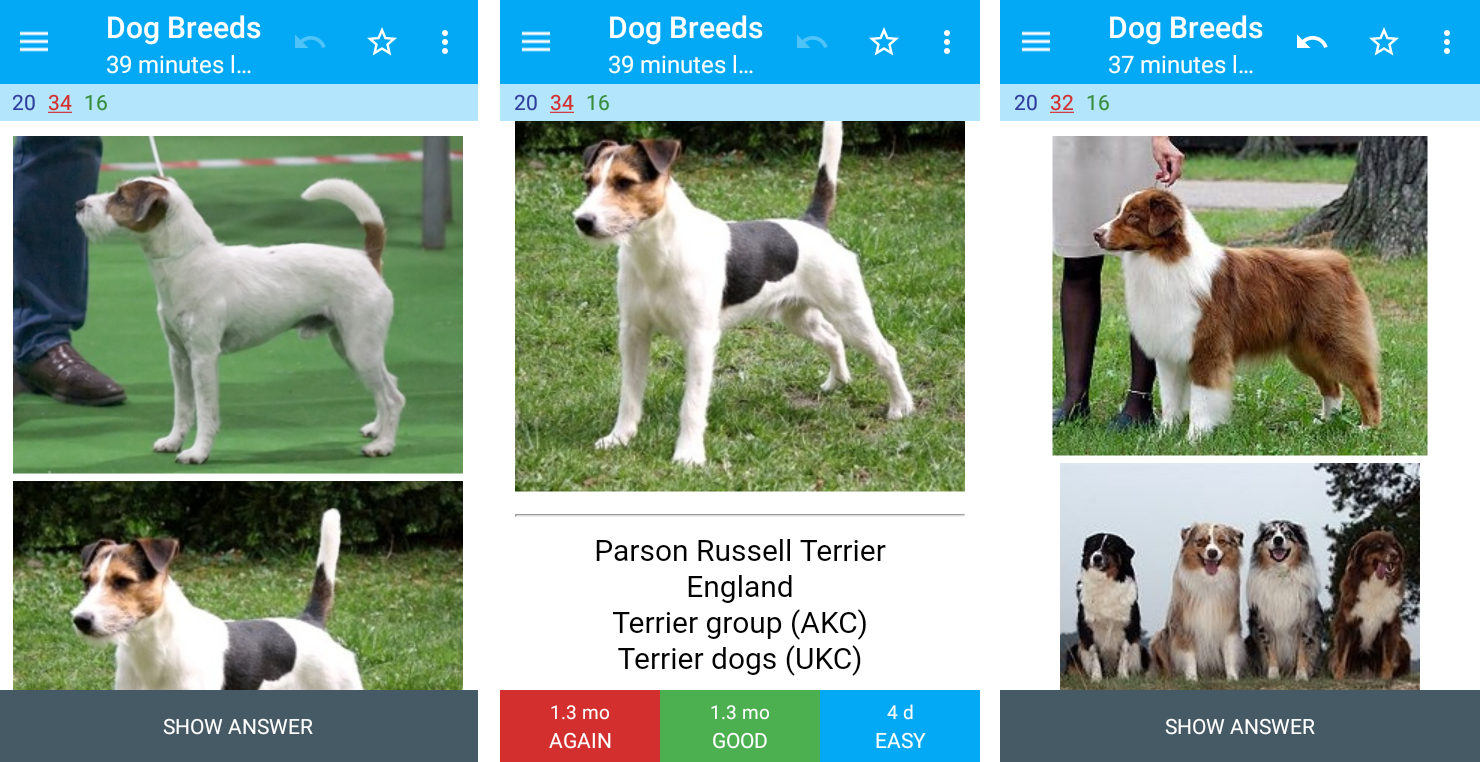
\includegraphics[scale=0.28]{./Figures/reviewer.png}
            \caption{Flashcard reviewer showing the front, back, front flow.}
            \label{fig:front-back-assess}
        \end{center}
    \vskip -5mm
\end{figure}

Many other secondary components are developed around the revision of flashcards, with the deck picker as the most relevant one. This component is the first contact users have with the application. Its main role is displaying the available decks of flashcards as seen in Figure \ref{fig:deck-picker}. It also allows several actions on the decks including selection, deletion, and addition. When users select a deck, the application starts the flashcards revision process. The deck picker connects to other parts of the application like statistics and settings. Finally, the deck picker displays other information including the number of flashcards and the time reviewing them.

\begin{figure}[htb]
    \vskip 5mm
        \begin{center}
            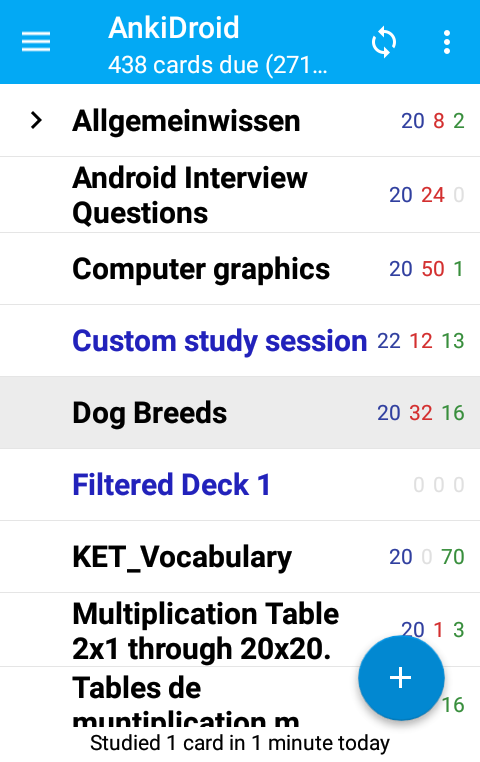
\includegraphics[scale=0.4]{./Figures/picker.png}
            \caption{Deck picker showing the decks of flashcards.}
            \label{fig:deck-picker}
        \end{center}
    \vskip -5mm
\end{figure}

The visual and logic characteristics of the flashcard reviewer and the deck picker were used to facilitate the inclusion of game elements and schemes. Visually, both elements present a structure that allows a smooth incorporation of new elements that do not interfere with their main purpose. In regard to logic, the deck picker allows getting access to new components of the application. On the other hand, the flashcard reviewer has a flow of events that can be linked to additional actions, which could provide instant feedback to users.

%----------------------------------------------------------------------------------------
\section{Initial gamification strategy}
\label{desi-gamification-strategy}
The process started with the definition of a model of extrinsic motivation based on rewards \citep{richter2015studying}. The basic tangible component of this model had the form of points, which were tied to the revision of flashcards. The approach was extended to include coins as an additional reward element that complemented the role of points. Points and coins presented characteristics that allowed them to be used beyond the reward model. However, coins differed from points on how they could vary in number and the way users could use them.

The model of motivation was extended to include more advanced game elements built upon the basic rewards. It incorporated a set of achievements that was defined based on the number of points. The achievements were also set to provide a more game-like mood to the overall user experience. Later, a customisation scheme made use of the characteristics of points to link them to achievements. Points along with customisation were also used to define a social and competition scheme. Additional elements were defined to keep users informed about their progress.

%----------------------------------------------------------------------------------------
\subsection{Rewards}
In games, a reward is something given to a player as the result of executing a task. In many cases, the objective is to motivate the player to do the same task again. In addition, rewards can also be defined as resources for later use; therefore, they can be accumulated. Based on this scheme, a virtual currency was defined in the form of coins. Since the core of the application was the revision of flashcards, such coins were given to users each time a flashcard was reviewed. Specifically, the number of available coins was increased each time the user assessed a flashcard.

A reward scheme requires the benefit the player receives to be proportional to the effort done. The content of the flashcards varied from one deck to another; it could be as simple as text, or as complex as images and audio. Therefore, the effort exerted in each flashcard was different. Thus, the number of coins granted in each flashcard was defined by the amount of effort. The most suitable way to calculate the effort of users based on the content of flashcards was by measuring the time spent on them. Hence, the number of coins per flashcard was defined as a function of time. However, a couple of restrictions had to be considered to avoid undesired behaviours from users.

Given that coins were also resources, users could be tempted to obtain them with minimal effort. One potential misbehaviour was passing flashcards as fast as possible to obtain the highest number of possible coins. Moreover, users could intentionally spend more time reviewing flashcards to obtain more coins. Diminishing these issues required setting ranges of time. Therefore, there were three ranges to calculate the number of coins in each flashcard: null, linear, and constant. The null range was one second long and started the moment a question or an answer was displayed. The linear range was three seconds long, and the number of coins was proportional to the amount of time. Finally, the constant range lasted until a new answer or question was displayed and no coins were given.

\begin{equation}
  c(t) =
      \begin{cases}
        0 & \text{if t $\leq$ 1}\\
        t & \text{if 1 $<$ t $\leq$ 3}\\
        3 & \text{if t $>$ 3}\\
      \end{cases}
    \label{eq:coins-formula}
\end{equation}

Equation \ref{eq:coins-formula} describes the calculation of coins, where \textit{c} is the number of coins as a function of the elapsed time in seconds, \textit{t}. The number of coins was always an integer value. It is important to note that there were minimum and maximum numbers of coins that could be earned in each flashcard, 0 and 6 (3 for the question and 3 for the answer) respectively. A potential drawback when calculating coins was the repetition of a flashcard since AnkiDroid allows undoing the previously reviewed flashcard. Therefore, users could earn additional coins for the same flashcard. However, reviewing a previous flashcard again was not penalised, and the previously earned coins were kept.

Coins could be spent by users to get benefits that will be explained later. This dynamic characteristic and how they were calculated could potentially reduce their potential benefits as rewards. Thus, it was necessary to implement a new element with a similar earning scheme but additional characteristics. Points are common elements in games. Their objective varies from context to context, but usually, they are used as additional rewards and provide information about progress since they are accumulative. Other educational platforms have added points as a motivational element \citep{disalvo2014khan}.

Points were designed to be calculated in a similar way to coins. There existed ranges of time to earn coins. The first range had the same objective as the one for coins, so, its duration was similar. A second range was meant to earn coins proportionally to the time; however, the relation is not linear but logarithmic as seen in Equation \ref{eq:points-formula}, where \textit{p} is the number of points as a function of the elapsed time in seconds, \textit{t}. Since logarithms are negative for values less than one, a max function between 1 and the logarithm was applied to avoid negative points. Finally, the number of coins was always an integer.

The logarithmic relation and the lack of a limit for points had two objectives. First, the creation of an additional distinction between points and coins. If the number of coins and points in a flashcard were greater than 0, it was unlikely that they were the same value. The second goal had to do with the limit for coins. Since the content of some flashcards could require more time than usual to review, the maximum number of coins per flashcard acted as a penalisation for flashcards with large content. Therefore, the lack of a limit for the number of points earned in a flashcard compensated for the coins penalisation in large flashcards.

\begin{equation}
  p(t) =
      \begin{cases}
        0 & \text{if t $\leq$ 1}\\
        max(1, 10log(t)) & \text{if t $>$ 1}\\
      \end{cases}
    \label{eq:points-formula}
\end{equation}

%----------------------------------------------------------------------------------------
\subsection{Achievements}
Rewards are by nature obtained after doing small tasks. Several games implement more advanced elements that increase the players' motivation; they are known as achievements. They are similar to rewards, but the main difference is the size of the tasks to get them. Those tasks usually require more time, the execution of a sequence of steps, or the repetition of smaller tasks. The most basic task in AnkiDroid is the revision of flashcards, which served to define the achievements scheme; moreover, the accumulative nature of points was also useful in the design.

In the solution, the achievements were designed to be obtained after the repetition of a small task (revision of flashcards). The number of points was used as the element to inform users of the progress to reach each achievement. Unlike rewards like coins or points that do not have a limit, achievements were defined as a set of specific elements to be gotten with a specific number of points. Therefore, users were aware of the number of available achievements and the required points to obtain them. Moreover, the application provided information about the reached achievements and the remaining ones.

In addition, to give AnkiDroid a more game-like mood, achievements were depicted as pets to be rescued. Those pets were called ankimals, a term that merges the words Anki and animals to provide a sense of identity with the application. The feeling of rescuing pets was complemented with notifications to inform users when a new ankimal was freed. The notifications were designed to encourage the users to rescue more pets by earning more points; therefore, they indirectly asked users to review more flashcards as seen in Figure \ref{fig:ankimals-rescue}.

\begin{figure}[htb]
    \vskip 5mm
        \begin{center}
            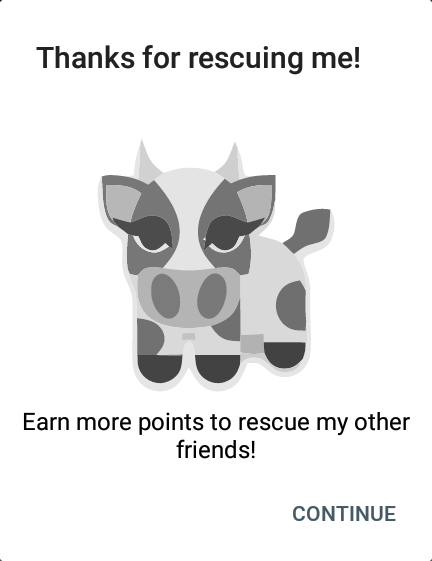
\includegraphics[scale=0.35]{./Figures/achievement_notification.png}
            \caption{Notification shown to user when achievement is reached.}
            \label{fig:ankimals-rescue}
        \end{center}
    \vskip -5mm
\end{figure}

%----------------------------------------------------------------------------------------
\subsection{Customisation}
Games provide customization aspects to give a more personal experience to players. In the solution, this scheme was defined with two elements. The first one was a nickname that could be set by the user. This element was meant to give a higher sense of participation within the application. The second aspect of a more personal experience was an avatar. It was meant to provide a visual representation of a player, which helped to create a sense of individuality. Both elements aimed at creating a sense of identity, but they differed in levels of customisation and constraints.

Nicknames were quite customisable and flexible. The only restriction was the maximum number of characters (12). Users were able to set their nicknames at any point. On the opposite, avatars were limited to some images, and users were required to get a number of points and icons. Unlike some games and applications where users can use any image to set an avatar, the application allowed users to choose one of the rescued ankimals. Moreover, since coins were defined as resources, users needed to spend a number of them to set ankimals as their avatars as seen in Figure \ref{fig:ankimals-select}. An additional level of customisation permitted users to colour ankimals since they were originally depicted in greyscale.

\begin{figure}[htb]
    \vskip 5mm
        \begin{center}
            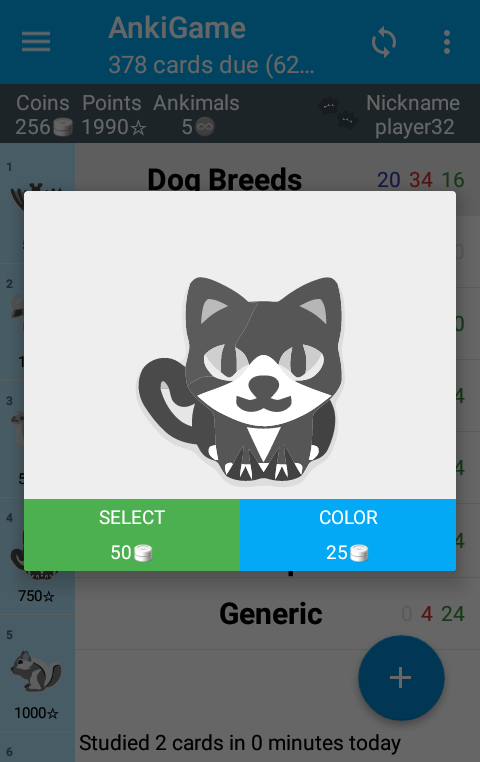
\includegraphics[scale=0.4]{./Figures/ankimal_selection.png}
            \caption{Dialog to select and color a rescued ankimal.}
            \label{fig:ankimals-select}
        \end{center}
    \vskip -5mm
\end{figure}

%----------------------------------------------------------------------------------------
\subsection{Social and competition}
The informative nature of points was also used to integrate another common element of games: leaderboard. In the solution, the leadearboard had two objectives. First, it provided a social context to the users. Thus, they knew that there were other people using the application. The social context was boosted with the inclusion of nicknames and avatars as seen in Figure \ref{fig:leaderboard}. That meant users could have a broader context of their identities within the application. Not only were they able to define their nicknames and avatars, but the leadearboard also provided a way to see others'.

The second objective of the leadearboard was aimed at adding a new level of motivation for the revision of flashcards. Since positions in the leadearboard depended on the number of points, users needed to review more flashcards to increase the number of points, hence, improve their positions. In addition, the positions were depicted as chess pieces, which could be interpreted as achievements. However, unlike rescuing ankimals, reaching a position in the leadearboard was not definitive. A position in the leaderboard could be lost against other users.

\begin{figure}[htb]
    \vskip 5mm
        \begin{center}
            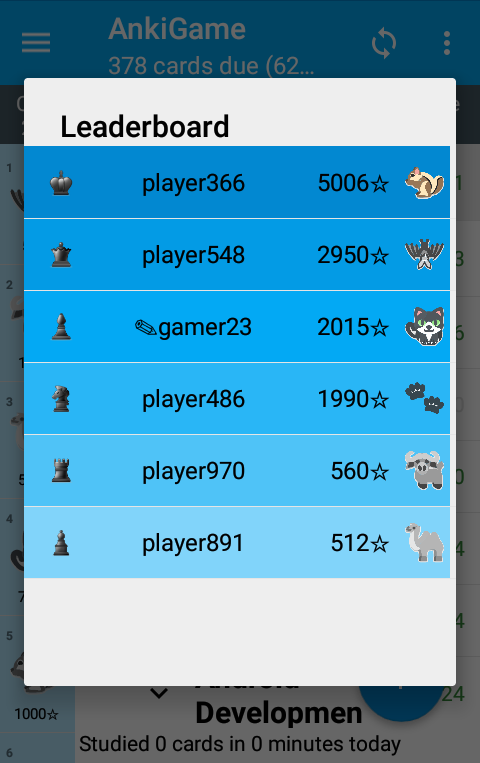
\includegraphics[scale=0.4]{./Figures/leaderboard.png}
            \caption{leadearboard showing the nicknames and avatars of users.}
            \label{fig:leaderboard}
        \end{center}
    \vskip -5mm
\end{figure}

%----------------------------------------------------------------------------------------
\subsection{Progress}
It was necessary to keep users informed about the state of the new gamification elements of the application. Similar to games that provide elements to inform about progress and other aspects, the solution added a status bar to provide information about the points, coins, rescued ankimals, avatar, and nickname. This new visual element was designed to be easily integrated into relevant parts of the application as seen in Figures \ref{fig:reviewer-modified} and \ref{fig:progress}, where it is located and constantly visible below the main bar of the application. Moreover, the design allowed instant updates of its elements.

\begin{figure}[htb]
    \vskip 5mm
        \begin{center}
            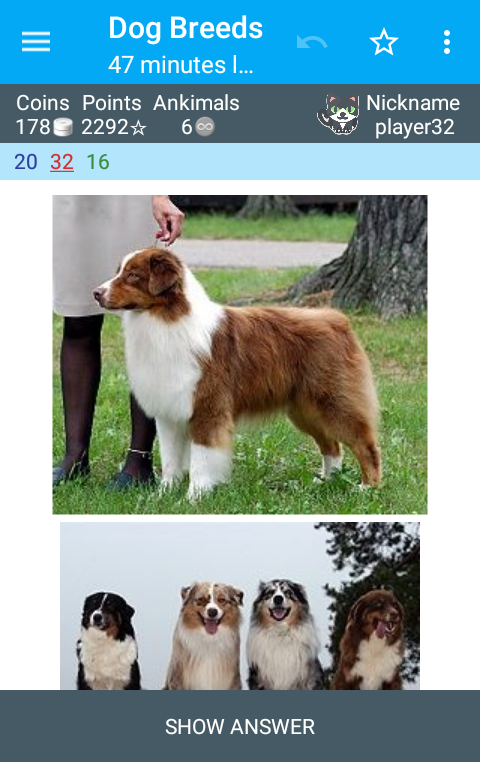
\includegraphics[scale=0.4]{./Figures/modified_reviewer.png}
            \caption{Modified flashcards reviewer displaying informative gamification elements.}
            \label{fig:reviewer-modified}
        \end{center}
    \vskip -5mm
\end{figure}

Additionally, a list of elements was also added in the deck picker to show the rescued and not rescued ankimals as seen in Figure \ref{fig:progress}. The list had the same informative purpose of the status bar; however, they differed in the interactions. While the status bar did not enable any kind of interactions, the list allowed users to pick any ankimal to set it as their avatar or add colour to it. The interactive nature of the list of ankimals was consistent with the list of pickable decks. Moreover, they shared the same vertical layout.

\begin{figure}[htb]
    \vskip 5mm
        \begin{center}
            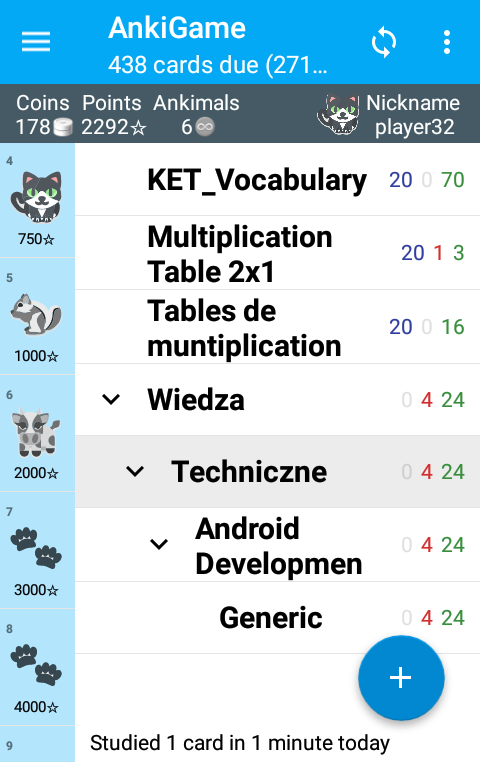
\includegraphics[scale=0.4]{./Figures/progress.png}
            \caption{Modified deck picker displaying informative gamification elements.}
            \label{fig:progress}
        \end{center}
    \vskip -5mm
\end{figure}

%----------------------------------------------------------------------------------------
\section{Game integration}
\label{game-integration}
The most important design decision in the solution was the inclusion of a game. The integration of a game was the key difference with other gamification approaches. Unlike the previously described elements that added new features to existing functionalities, a game was a completely new component in the application. Therefore, it was required that the game be easy to play and avoided an unnecessary level of complexity. For this reason, a casual game was the most suitable option. Casual games are straightforward and their gameplays allow short periods of play, which convert them into activities that can be executed during work or study breaks.

The game needed to be integrated into AnkiDroid in a way that it fitted in the structure easily. Moreover, the integration required the definition of a linkage between the game and other components of the application. These conditions set the scenario to modify the game and use the previously described gamification elements. The final design set the game as a component with some flexibility to use and smoothly connected to the rest of the application. However, the design also included some constraints aimed at increasing the user engagement of flashcards revision.

%----------------------------------------------------------------------------------------
\subsection{Modifications to the game}
2048 is a simple yet challenging game due to the high number of turns to form the block 2048 (1024 turns in the perfect case). Another aspect that increases the difficulty of the game is the limited space. If there are no more empty cells in the grid, and no further movements are possible, then the game is over. Such difficulty along with the need to connect the game with the rest of the application set the starting point to modify the game. Such modifications had to be consistent with the easy-to-use paradigm of casual games. Moreover, they needed to maintain a consistency such that their behaviour and results were easy to understand.

Based on the requirements to modify the game, a set of elements was defined to ease the gameplay. Those elements took the form of cheat tricks aimed at providing more alternatives to win. Each trick changed the state of the grid so that players had more options in a next move. The state of the grid was defined by the positions of the blocks and their values at a given turn. Therefore, there existed several approaches to change the state of the board. Moreover, each trick needed to provide a different degree of benefit; thus, they were not equally valuable. The modifications included four cheat tricks as seen in Table \ref{tab:tricks}. It is important to note the restrictions to use them based on the state of the grid.

\begin{table*}[!htb]
  \centering
  {\renewcommand{\arraystretch}{2}
    \begin{tabular}{|R{2cm}|R{6cm}|R{5cm}|}
    \hline
    \multicolumn{1}{|>{\centering\arraybackslash}m{2cm}|}{\textbf{Name}} &
    \multicolumn{1}{>{\centering\arraybackslash}m{6cm}|}{\textbf{Benefit}} &
    \multicolumn{1}{>{\centering\arraybackslash}m{5cm}|}{\textbf{Usage conditions}}\\
    \hline
    Gift & Adds a randomly positioned block that can merge with any block whose value is less than 512. & There is at least one empty cell in the grid.\\
    \hline
    Doubler & Doubles all the blocks whose values are 2. & There is at least one block with a value of 2 in the grid.\\
    \hline
    Remover & Removes all the blocks whose values are 2. & There is at least one block with a value of 2 in the grid. \newline There is least one block with a value greater than 2.\\
    \hline
    Undo & Undoes the last movements (up to 10 previous movements). & There are previous movements.\\
    \hline
    \end{tabular}
  }
  \caption{Cheat tricks for the game, their benefits, and usage conditions.}
  \label{tab:tricks}
\end{table*}

%----------------------------------------------------------------------------------------
\subsection{Connection with flashcards revision}
A connection meant finding existing elements in AnkiDroid that could act as the glue material between the game and the revision of flashcards. In other words, the connection had to be done to include a motivational aspect to encourage users to review more flashcards to obtain benefits in the game. Thus, the user engagement could increase by adopting elements from AnkiDroid to the logic and structure of the game. The original application did not present elements that could be easily adjusted to the game. However, two of the gamification elements defined earlier provided a way to make the connection.

The first elements were points, which already provided a motivational aspect in the revision of flashcards. The informative nature of points was previously used to define achievements in the revision of flashcards. Following the same scheme, they were also used to define achievements in the game. In this case, the cheat tricks in the game were linked to a specific number of points based on the benefits they provided; the higher the benefit, the higher the number of points. Therefore, the tricks were initially hidden, then, users needed to obtain the corresponding number of points to reveal each trick. Finally, unlike ankimals, users were not notified when a trick was revealed since the main interest was the revision of flashcards, not playing the game.

The number of available tricks was small (4), and revealing each of them was a one-time event. This situation could potentially limit the connection between the game and the revision of flashcards. Therefore, it was necessary to take advantage of coins, which were already used as resources to select and colour ankimals. In the game, once the tricks were revealed, players could use them at any point as long as they had the required number of coins. In some sense, users needed to buy tricks with the coins they earned reviewing flashcards. Similarly, a specific number of coins was set for each trick based on the benefit level as seen in Table \ref{tab:tricks-coins-points}.

\begin{table*}[!htb]
  \centering
  {\renewcommand{\arraystretch}{2}
    \begin{tabular}{|R{3cm}|R{3cm}|R{2cm}|R{2cm}|}
    \hline
    \multicolumn{1}{|>{\centering\arraybackslash}m{3cm}|}{\textbf{Cheat trick}} &
    \multicolumn{1}{>{\centering\arraybackslash}m{3cm}|}{\textbf{Benefit level}} &
    \multicolumn{1}{>{\centering\arraybackslash}m{2cm}|}{\textbf{Points}} &
    \multicolumn{1}{>{\centering\arraybackslash}m{2cm}|}{\textbf{Coins}}\\
    \hline
    Gift & Low & 100 & 10\\
    \hline
    Doubler & Medium & 500 & 20\\
    \hline
    Remover & High & 1000 & 30\\
    \hline
    Undo & Higher & 2000 & 40\\
    \hline
    \end{tabular}
  }
  \caption{Costs of cheat tricks in terms of points to reveal and coins to use them.}
  \label{tab:tricks-coins-points}
\end{table*}

%----------------------------------------------------------------------------------------
\section{User interface considerations}
Several user interface aspects were considered to implement the game elements described earlier. First, the modifications in the game required the addition of interactive elements for each cheat trick. Initially, colour information was used to differentiate the cheat tricks and to provide clues about their status (blocked, enabled, usable)  as seen in Figure \ref{fig:modified-game}. Moreover, since the gameplay required the users to slide vertically and horizontally, cheat tricks could easily be selected by mistake. Avoiding that problem required designing a translucent curtain to be removed by the user before selecting cheat tricks.

\begin{figure}[htb]
    \vskip 5mm
        \begin{center}
            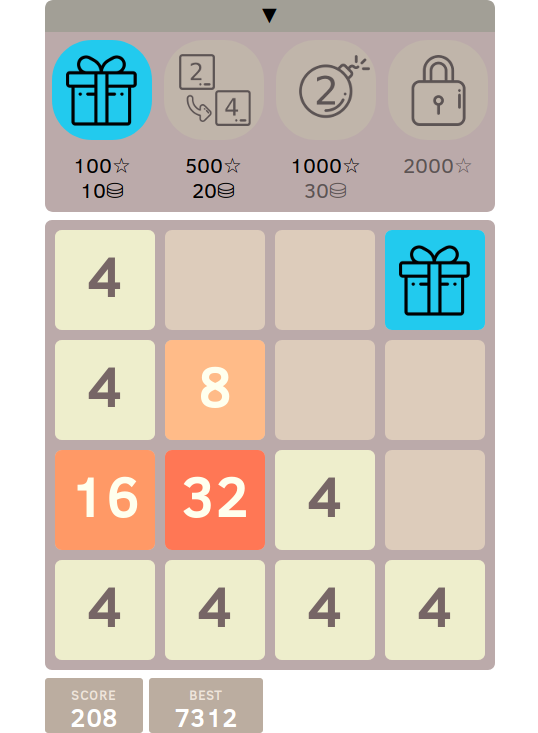
\includegraphics[scale=0.4]{./Figures/modified_game.png}
            \caption{Modified game showing the cheat tricks with different status at the top of the grid.}
            \label{fig:modified-game}
        \end{center}
    \vskip -5mm
\end{figure}

In AnkiDroid, the main considerations to implement the game elements were related to keeping consistency in the overall aspect of the application and the visual clues for the user. The first aspect required using the same colour scheme along with other elements like the font type and size. On the other hand, visual clues were meant to provide information about modifications in the game elements. This was done by implementing animations where necessary. For instance, when the number of coins or points changed, animations that updated the corresponding visual elements were implemented. Finally, the visual structure was maintained as much as possible to avoid the new components from being intrusive.

%  % Use this as criticism
%  Evidently, users could play the game without using tricks, but






